\chapter{Diffuse Polarisation}
\label{ch: Canals}

The previous two chapters have described the work I have done to increase the number of RM values found for extragalactic sources within the diffuse emission of the Galactic plane. This chapter showcases the results of the 3D rotation measure synthesis pipeline, and further analysis, which progresses our understanding of the diffuse polarisation within the Galaxy.

\section{Evolution of Diffuse Polarisation Measurements }

Characterising the polarisation of Galactic diffuse emission is a relatively new field, begun by work by \cite{Wieringa_1993}. This work found various structures present in observations of diffuse polarised emission. These observations were taken using the Westerbork Synthesis Radio Telescope (WSRT) at 325 MHz at high Galactic latitudes. These structures were seen on a variety of scales down to a few arcminutes and do not have an apparent counterpart in observations of total intensity. This work also compared these observations to numerical simulations of interferometric observations of a uniformly polarised background which suggested that qualitatively, this is a good description of the observations.

Further observations were taken by WSRT in the frequency range 341-375 MHz (e.g. \cite{Haverkornetal_2000}, \cite{Haverkorn_2001}, \cite{Haverkorn_2004}) which analyse in greater detail the structures present. 
%One key structure described are depolarisation canals. These canals are narrow, filament-like one dimensional structures and have a very low polarised intensity.
There has also been pioneering work done at lower frequencies by \cite{Bernardi_2009}. This work also used WSRT to characterise the foreground emission for epoch of reionisation experiments, probing an area of the sky at a low Galactic latitude within 140-160${\rm\,MHz}$. 

POSSUM has allowed us to probe more of the Galaxy as it uses higher frequencies, i.e. 943$\,{\rm MHz}$, and has pointings closer to the Galactic centre, meaning that the radiation observed has a longer path through the diffuse emission of the Galactic plane. Diffuse polarisation had not been seen before at such high frequencies as before ASKAP and MeerKAT, such high frequencies were not covered by synthesis arrays. Higher frequencies, and thus shorter wavelengths, result in a larger maximum scale of detectable structures in Faraday space as

\begin{equation}
    \phi_{max-scale} = \frac{\pi}{\lambda_{min}^2}
\end{equation}

(e.g. \cite{Sun_2015}). This in turn means that emission with wider peaks in FD can be detected and as more distant material will have a larger range of RM in a fixed beam size for a given RM gradient, and thus a wider FDF, this emission can be seen.

Another advantage of POSSUM is the smaller beam size, which means that the RM distribution can be better resolved. However, for the polarised emission to be visible, the RM gradients also have to be large enough to divide Stokes Q and U into small enough regions to detect on short baselines. This, combined with the limit in terms of FDF as described above are why the features that are visible in polarised intensity do not have corresponding features in total intensity.




%Another possible explanation for the depolarisation canals is a rapid switching between multiple peaks of RM. %I can remember reading something about this but I can't find it now - grr

%This quick change in RM value could result in a steep gradient, and if positioned in a certain way could produce canal like structures. %I'm like 90% sure what I've have just written is wrong!



\section{3D Pipeline}
\label{3d pipeline}

In order to investigate the diffuse polarisation of the field 1505-60 I first ran the 3D POSSUM polarimetry analysis pipeline

This implementation of this pipeline consists of three steps: creating the spectral model, 3D RM synthesis and peak fitting.

The first step fits a model to the Stokes I data cube using RM-tools' fitIcube routine. This script fits Stokes I models pixel-wise using the 1D fitting routine to the Stokes I data cube. This model cube is created using the same power law as used for the model Stokes I spectrum found for each source as part of the one dimensional pipeline.

The second step of the pipeline has two main parts. First it uses the model cube calculated to find the fractional polarisation and then it performing 3D RM synthesis which uses the rmsynth3D routine from RMTools to perform a non-gridded discrete Fourier transform, from Equation \ref{eq: discrete rm synth}, to calculate the FDF. The weighting of this data was chosen to be inverse variance again to reduce the noise in the FDFs. 
The spacing between samples and maximum distance over which Faraday depth is defined is also calculated in the same way as for the 1D synthesis. 
The third and final step of this pipeline is peak fitting. This step uses the RMpeakfit$\_$3D routine from RM-tools to apply the one 
dimensional RM spectrum characterisation and peak fitting techniques using the same method as the peak fitting described in the extract spectra step of the one dimensional pipeline and then applies it pixelwise to the three dimensional FD cube. This step produces 2D maps of rotation measure and polarised intensity.

Descriptions of the outputs of this pipeline can be found in Appendix \ref{AppA: 3D pipeline output}.

The results of the 3D polarimetry analysis pipeline on the field EMU1505-60 yielded a 2D map of the peak polarised intensity, Figure \ref{fig: pi map}, and rotation measure, Figure \ref{fig: rm map}. 

\begin{figure}
    \centering
    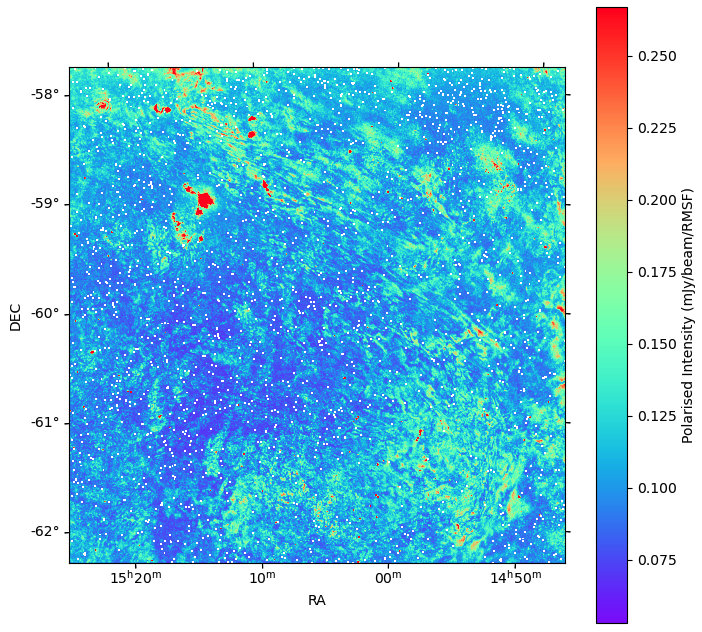
\includegraphics[width=1\linewidth]{Thesis_Template//Figures/Pi map.png}
    \caption{Polarised Intensity Map of EMU1505-60}
    \label{fig: pi map}
\end{figure}

\begin{figure}
    \centering
    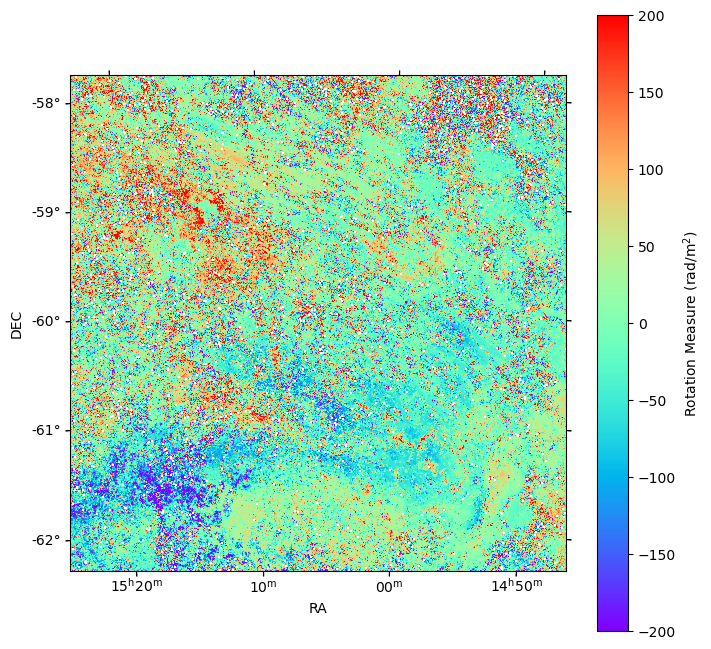
\includegraphics[width=1\linewidth]{Thesis_Template//Figures/RM map.png}
        \caption{Rotation Measure Map of EMU1505-60}
    \label{fig: rm map}
\end{figure}

Figure \ref{fig: pi map} demonstrates that there is polarised emission present across the entire field, which is interesting as it does not match the structure and distribution of the total intensity. The whole field is full of smooth, high-brightness diffuse synchrotron emission, visible in single-dish maps. This is resolved out in this synthesis image, leaving only structures with scales less than half a degree. The Faraday effect breaks up the polarised intensity, making it more unstructured, which can be seen as the 'blobby' pattern, most prominent across the right hand side of the image (see Figures \ref{fig: blobby zoom} and \ref{fig: canals zoom}). The supernova remnant MSH15-22 can be seen clearly in the upper left corner of the image as an extended peak in polarised intensity and can be seen in more detail in Figure \ref{fig: sn zoom}.

\begin{figure}
    \centering
     \begin{subfigure}[b]{\textwidth}
        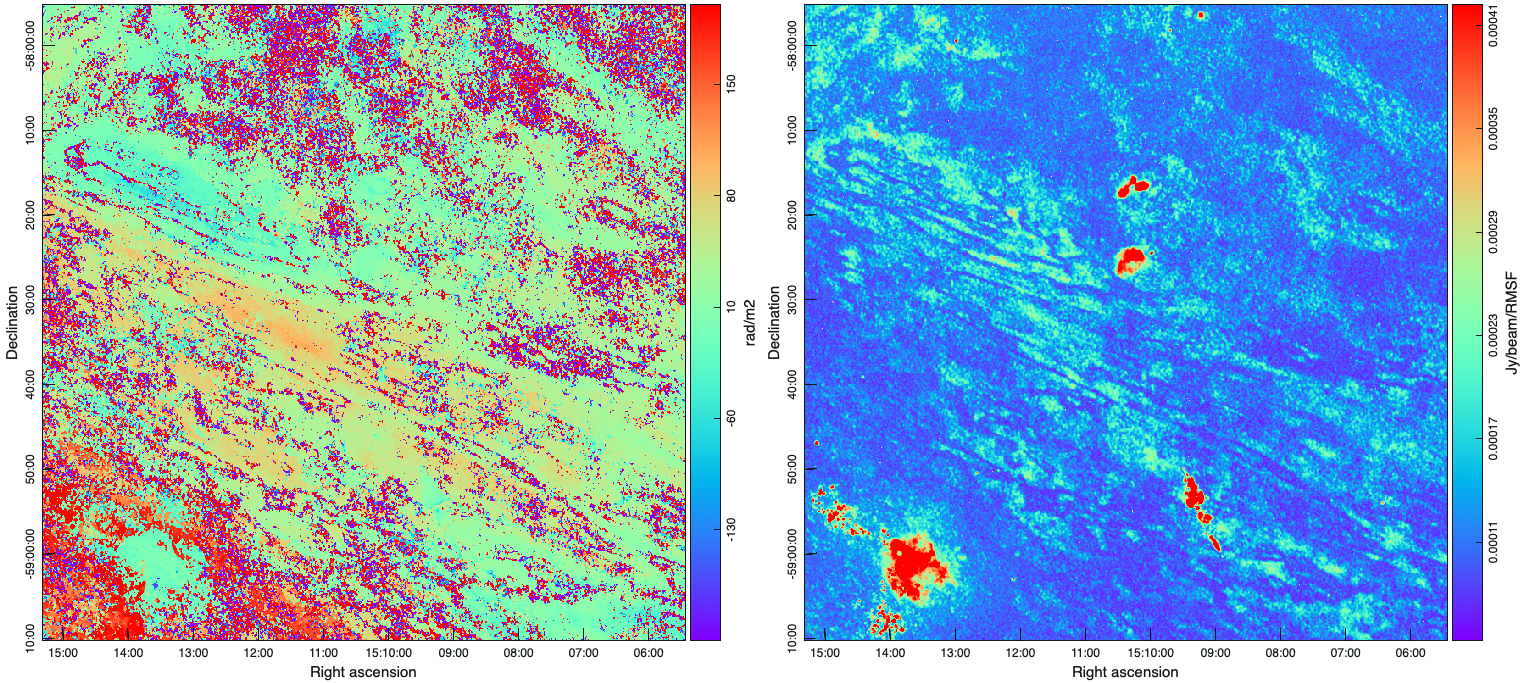
\includegraphics[width=\linewidth]{Thesis_Template/Figures/RM_PI top right.png}
        \caption{Structure dominated by long filament like canals which can be seen in both RM and PI maps}
        \label{fig: canals zoom}
    \end{subfigure}

    
    \vspace*{0.05cm}

    
    \begin{subfigure}[b]{\textwidth}
        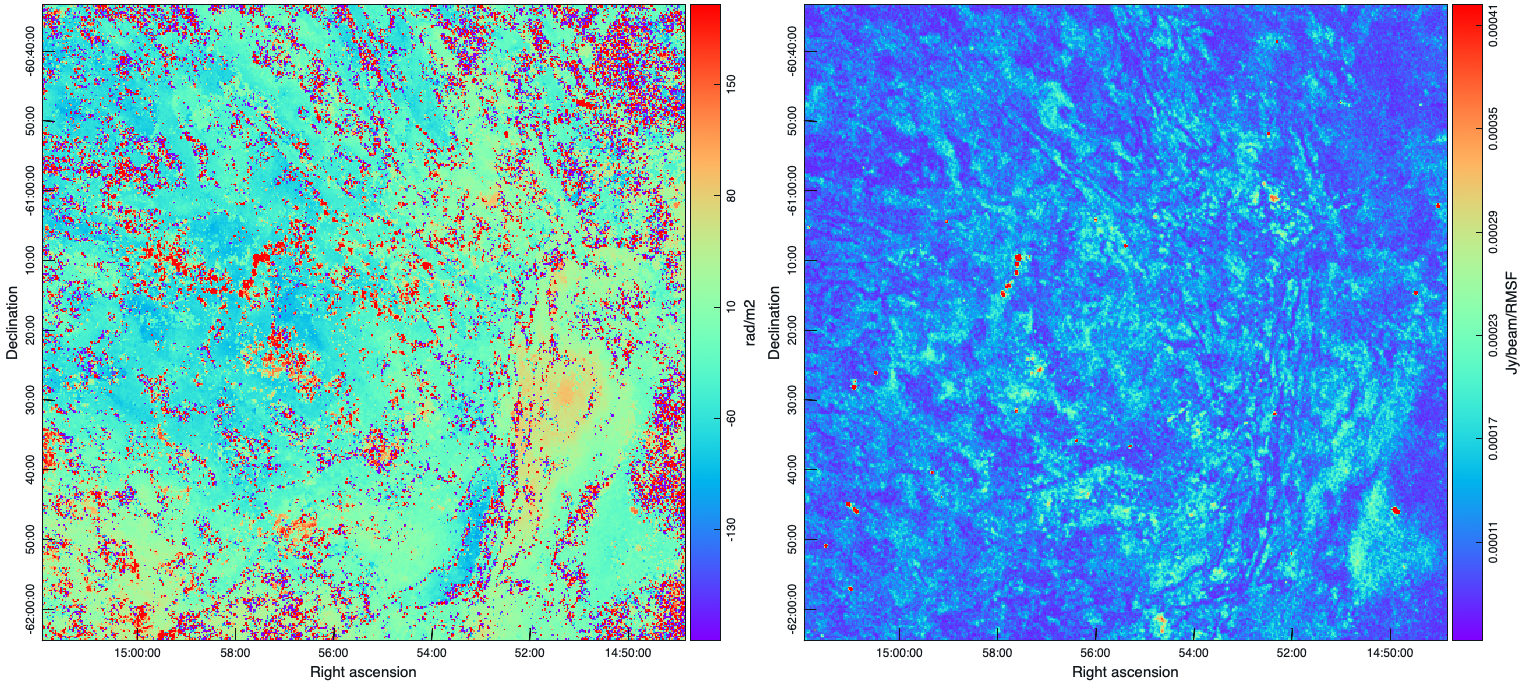
\includegraphics[width=\linewidth]{Thesis_Template/Figures/RM_PI bottom right.png}
        \caption{Blobby structure can be clearly seen in the PI map, with varying corresponding RM. Canal-like structure can also be seen in this region}
        \label{fig: blobby zoom}
    \end{subfigure}

    
    \vspace*{0.05cm}

      \begin{subfigure}[b]{\textwidth}
        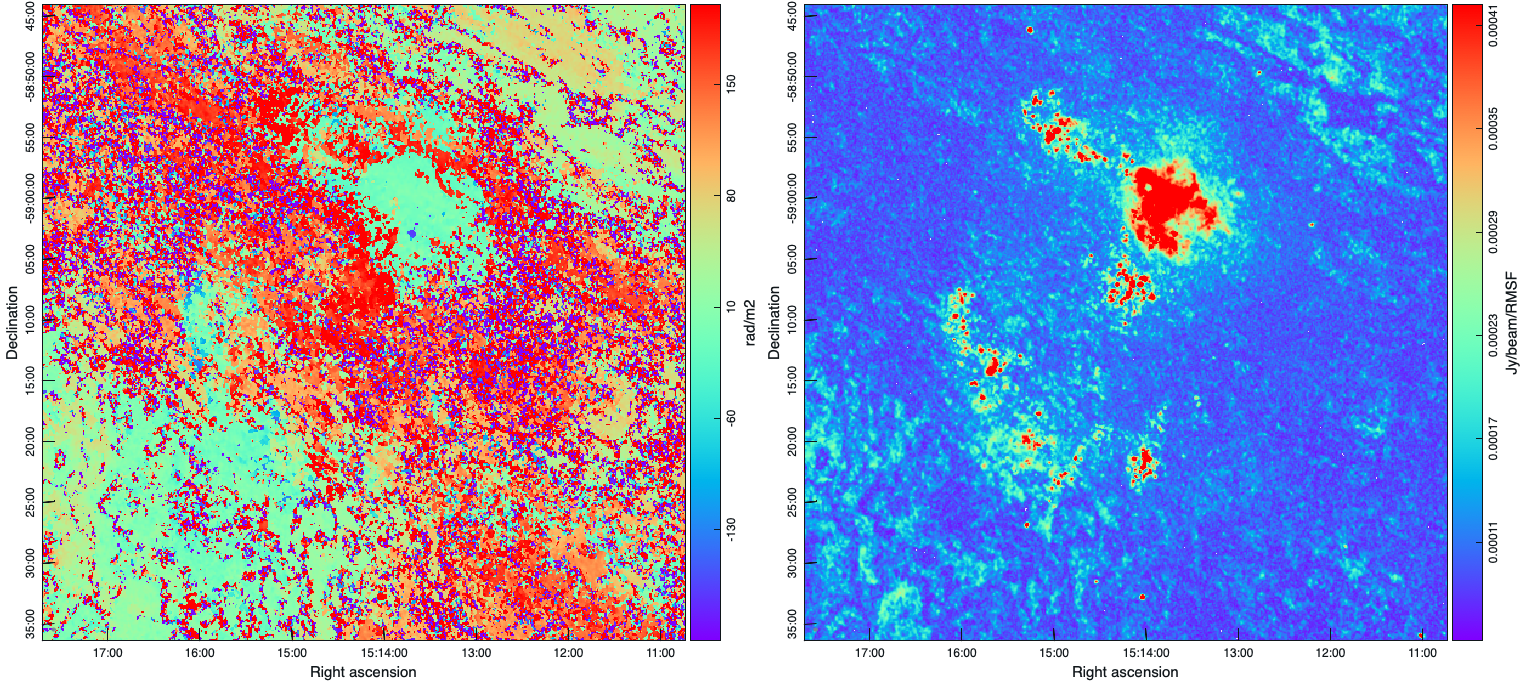
\includegraphics[width=\linewidth]{Thesis_Template/Figures/RM_PI_MSH 15-22.png}
        \caption{Supernova remnant MSH 15-22, which can be seen as a peak in the PI map, but has a low magnitude in the rotation measure map}
        \label{fig: sn zoom}
    \end{subfigure}
    

   
    
    \caption{Zoomed in figures of interesting features in Rotation measure (left) and Polarised Intensity (right) maps for field EMU1505-60}
    \label{fig:pi and rm zooms}
\end{figure}



This map has not been corrected for Ricean bias, which is a positive bias which arises from the contribution of the difference between the measured and true values for Stokes Q and U. However, as I have blanked all values with a signal to noise below 2, the contribution of this bias is minimal.

Another interesting feature which can be seen in both these Figure \ref{fig: pi map} and Figure \ref{fig: rm map} is canal like structures, particularly in the upper right hand quadrant of the polarised intensity map (see Figure \ref{fig: canals zoom}). Canal-like structures have also been identified in many other POSSUM fields by Dr Jennifer West (priv. comm.).

These canals are parallel to the Galactic plane, which means that they are parallel to the projected magnetic field of the Galaxy, as measured by \cite{Planck_XXV}. They also run parallel between the RM and PI maps, which implies that the RM gradient is perpendicular to the canals. Further quantitative analysis of the RM gradient is described in Section \ref{grad analysis}. There have been two predominant explanations for these canals put forward. One proposed by \cite{Haverkornetal_2000} suggests that beam depolarisation is responsible. Beam depolarisation is caused when the polarisation angle varies significantly within a beam such that for each line of sight there is a complementary line of sight that has the same polarised intensity, but the polarisation angle is shifted by 90$^\circ$. This was believed to be the case because it was found that the polarisation angle changes by 90$^\circ$ across the beam. This does not account for why the patterns of canals vary with wavelength.

The other is that they are instead caused by differential Faraday rotation in the interstellar medium. %\cite{beck}. 
\cite{Shukurov_and_Berkhuijsen_2003} built on this theory by proposing that the canals are in fact due to multiples of RM where $RM = RM_0 \equiv n\pi / (2\lambda^2)$ with $n$ being integer multiples. Their model follows Burn's sinc law (\cite{burn_1966}) which is zero when the intrinsic Faraday rotation is rotated by exactly $\frac{\pi}{2}$, $\frac{3\pi}{2}$ etc. This model would mean that the depolarisation varies more smoothly as the width of the canal is set by the RM gradient, rather than the beam size.

\section{Structure Detection}

Before conducting further analysis on the structure within these maps it is important to verify that the structure is that the interferometric observation has not fully detected this structure and that it is in fact just an artefact of the observational technique, such as the large fractional variations in Stokes Q and U observed could instead actually be small perturbations on a very smoothed polarised structure that has been resolved out. If this were the case, the polarisation angles would be much more uniform over the field (\cite{Haverkorn_2004}). In order to investigate this further, I conducted the 3D RM synthesis on the same field, EMU1505-60, but with only the lowest 100 frequency channels, which have a $\lambda^2$ range of between 0.11-0.14$\,$rad$\,$m$^{\shortminus2}$. The full frequency range gives a corresponding $\lambda^2$ range of 0.076-0.14$\,$rad$\,$m$^{\shortminus2}$. If this structure has not been fully detected, it should be better detected at lower frequencies because larger changes in angle for a given RM gradient would be more likely to remove the large-scale component which we can't detect, but would change the RM map. Therefore, by comparing the full band and the lower section of the band, we will be able to see the completeness of this structure. 

I compared the rotation measure and polarised intensity across the entire frequency range to the lower frequency range by creating Figures \ref{fig: rm vs lower} and \ref{fig: pi vs lower}. These plots only show values for which the error of the lower frequency range is less than 3 rad$\,$m$^{\shortminus2}$, which leaves 39$\%$ of the total number of pixels.

\begin{figure}
    \centering
    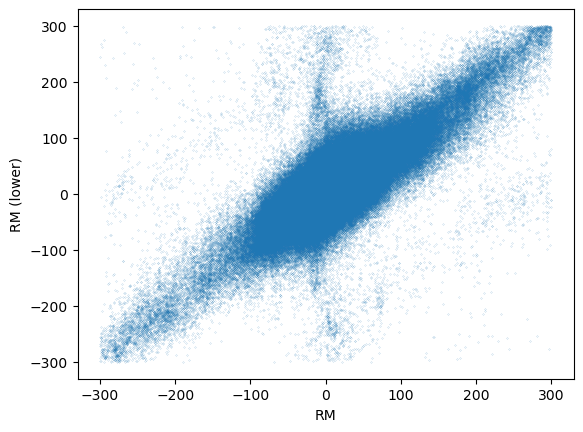
\includegraphics[width=1\linewidth]{Thesis_Template/Figures/RM_vs_lower.png}
    \caption{Plot of rotation measure across the full frequency channel range in rad$\,$m$^{\shortminus2}$ against the polarised intensity across the lowest hundred frequency channels.}
    \label{fig: rm vs lower}
\end{figure}

\begin{figure}
    \centering
    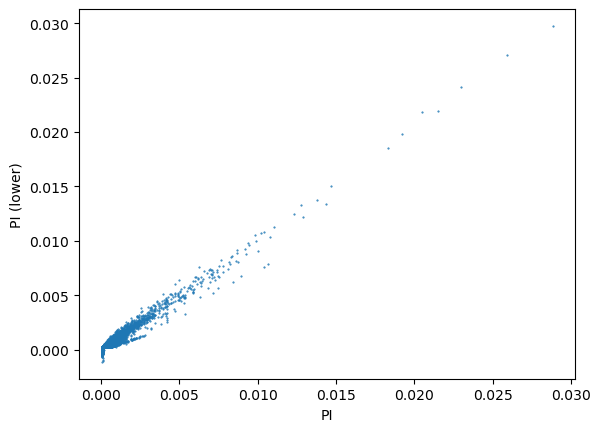
\includegraphics[width=1\linewidth]{Thesis_Template/Figures/PI_vs_lower.png}
    \caption{Polarised intensity across the full frequency channel range in Jy/beam/RMSF 
    against the rotation measure across the lowest hundred frequency channels.}
    \label{fig: pi vs lower}
\end{figure}

Both plots show a strong positive correlation with a gradient close to 1 between the full and the lower frequency ranges, which indicates that the same structure is detected in both the lower frequency section and across the complete frequency band. Therefore, this diffuse structure is real. Some outliers within RM can be seen around one in the full band, but with values across the whole range in the lower band. An explanation for this is still required as there is not an obvious cause for this, however these outliers make up only $0.2\%$ of the RM values.


\section{Peak Fitting}

There are two different broad categorisations of Faraday spectra: Faraday simple and Faraday complex (\cite{Alger_Livingston_McClure-Griffiths_Nabaglo_Wong_Ong_2021}, \cite{thomson2023rapidaskapcontinuumsurvey}, \cite{vanderwoude2024prototypefaradayrotationmeasure}). Faraday simple refers to spectra that have a single peak in the form of a delta function, which gives an unambiguous RM value. If there is more than one peak in the spectra, or the peak has a finite width, it is referred to as Faraday complex. One possible cause for Faraday complexity is multiple synchrotron emitting regions with different RMs along the same line of sight, for example, background and foreground emission from a supernova remnant. This would appear in the Faraday spectrum as multiple peaks or a Gaussian broadening such that the peak cannot be resolved. A scenario such as this would lead to depolarisation. 

In order to investigate the occurrence of multiple peaks within the rotation measure, I utilised code written by Dr Vasu Shaw
to identify spectra with multiple peaks and make maps of the RM values of the individual peaks. 
%Where multiple peaks are found, they are ordered by magnitude, with the primary being the largest. 
The primary peak, Figure \ref{fig: peak 1}, was consistent with the result from the pipeline.

\begin{figure}
    \centering
    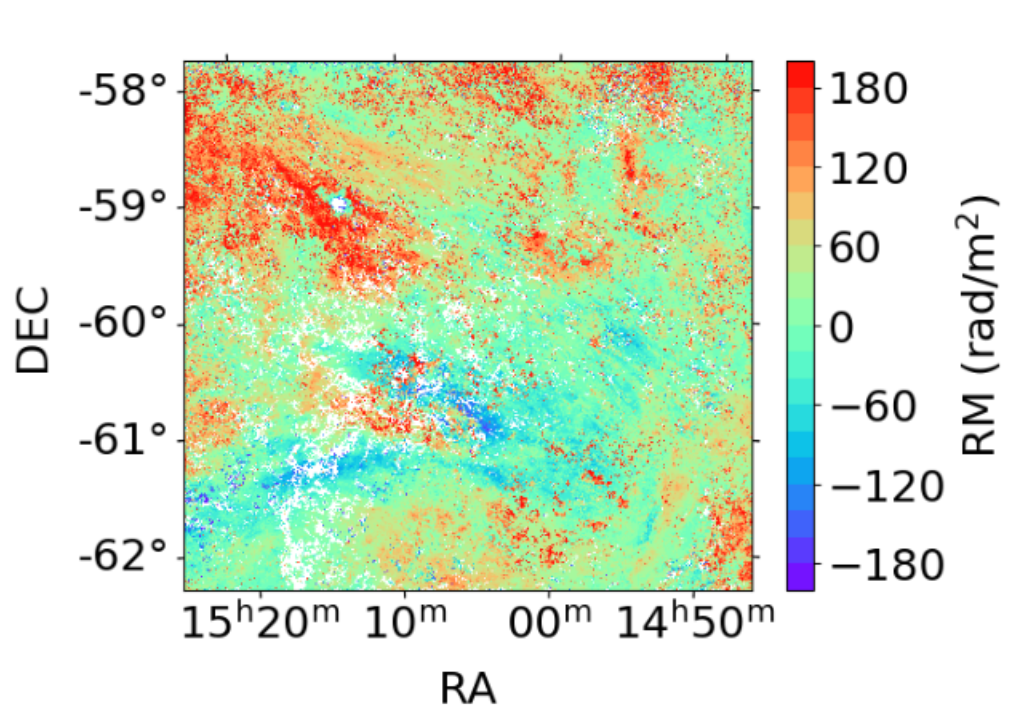
\includegraphics[width=\linewidth]{Thesis_Template/Figures/Peak 1.png}
    \caption{The primary peak in the FDF cube for field EMU1505-60.}
    \label{fig: peak 1}
\end{figure}


\begin{figure}
    \centering
    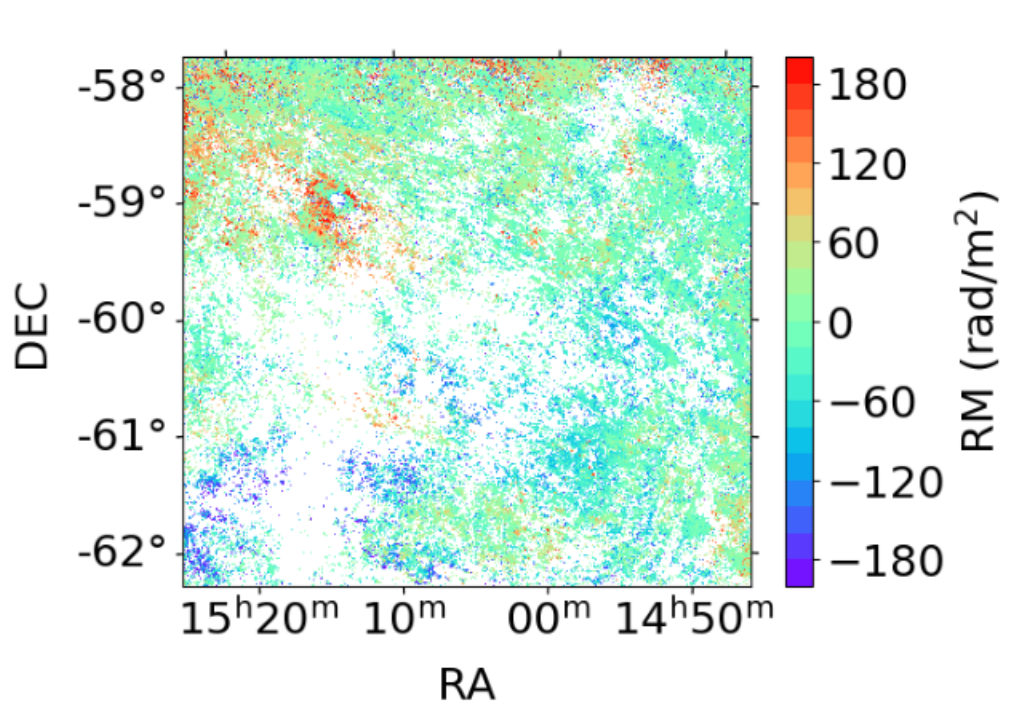
\includegraphics[width=\linewidth]{Thesis_Template/Figures/Peak 2.png}
    \caption{The secondary peak in the FDF cube for field EMU1505-60.}
    \label{fig: peak 2}
\end{figure}

\begin{figure}
    \centering
    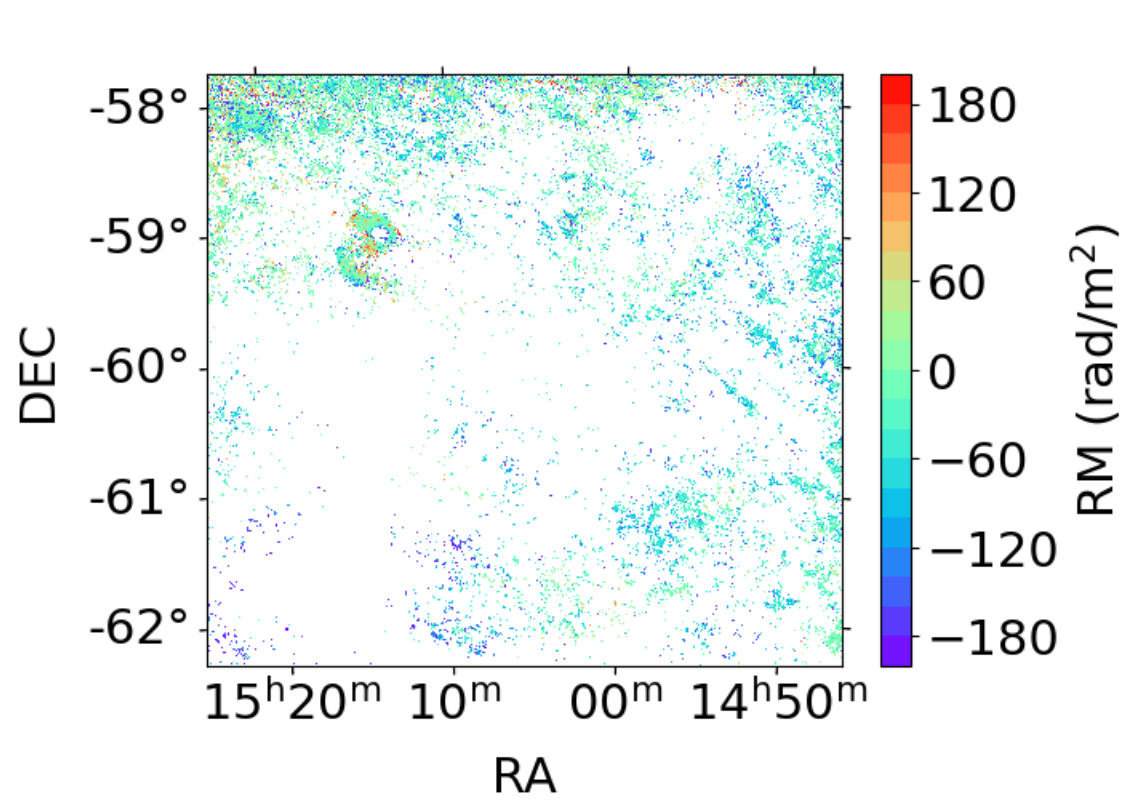
\includegraphics[width=\linewidth]{Thesis_Template/Figures/Peak 3.png}
    \caption{The tertiary peak in the FDF cube for field EMU1505-60.}
    \label{fig: peak 3}
\end{figure}

Figures \ref{fig: peak 2} and \ref{fig: peak 3} demonstrates that there are multiple peaks within the FDF cube. The secondary and tertiary peaks by visual inspection appear to have a similar value to the primary peak, which suggests that there is not a large difference between the peaks which could lead to a depolarisation canal to be seen. These results therefore do not support the explanation that multiple peaks are responsible for the canal phenomena.

For POSSUM, the maximum detectable scale for RM synthesis is smaller than the width of the RMSF, so such features as multiple peaks can't be clearly and correctly resolved. If the spread is less than the maximum scale, but not negligibly small, then FDF peak will be slightly wider than the RMSF. A broad FDF component will disappear if it is a smooth peak or produce peaks which are not real but in fact detections of the distribution edges (\cite{Erceg_2022}). This would explain why the multiple peaks observed are close to each other in FD.

\section{Gradient Analysis}
\label{grad analysis}

Conducting gradient analysis of the rotation measure cube allows for a more quantitative investigation of the canal features. One of the products of the complete POSSUM pipeline will be 3D RM synthesis images of the whole survey, and as part of this process RMclean (\cite{Heald_2009}) will be applied, which will reduce interference from the sidelobes of the RMSF. This step had not been done on the field previously analysed in this dissertation. Dr Roland Kothes has used a separate analysis of the publicly available Stokes I, Q and U cubes from POSSUM at low Galactic latitudes via the same process as the POSSUM pipeline, but without mosaicking the separate fields toegther as will be done for POSSUM. Also no correction for the ionospheric Faraday rotation has been made, however as this does not cause structure or depolarisation this lack of correction would not affect the outcome of this analysis. Therefore I have used on of these processed fields, EMU1615-64, to conduct gradient analysis. This field was chosen as it showed the most prominent example of the canal-like filaments of interest, however these structures could be seen in many POSSUM fields.

For this analysis I used NINER to apply gradient masks. I applied a gradient mask for North, East, South and West to the rotation measure map (which is shown in Figure \ref{fig:1615-64 rm}). These masks can be found in the NINER documentation\footnote{NINER documentation can be found at http://www.aips.nrao.edu/cgi-bin/ZXHLP2.PL?NINER} \footnote{A bug was found within NINER which has resulted in the masks producing gradients in the opposite direction to those expected. This was adjusted for manually.}. I then rotated averaged the opposite directions, i.e. North and South, East and West and then found the average between these pairings. Finally, I calculated the direction and magnitude of the gradient at each pixel. By normalising and using an HSV image, converting the direction into the hue value and the magnitude into a brightness value I created Figure \ref{fig:hue} to highlight the depolarisation canals. The bright areas in this figure show areas of large gradient, with the stripes of colour representing lines with a consistent angle of gradient. These can be seen at a variety of orientations with large magnitudes, especially within the centre of the image. The bright areas without extended gradient features are due to regions of low signal to noise where the jumps in RM are due to noise rather than true features. The black regions are regions with no value for RM and very low PI. By comparing this map to the PI map (Figure \ref{fig:1615-64 pi}) it can be seen that not all gradients found have a corresponding feature in PI. An example of a canal feature in PI corresponding to a change in RM and thus a clear gradient in the gradient map is shown in Figure \ref{fig: 1615 zoom}. The prominent feature in C, the green filament can be seen to correspond to the change between an RM of $\sim 175$ and $\sim 125\,$rad$\,$m$^{\shortminus2}$. This also partially corresponds to a canal in PI, however this does not follow the full line of change in RM.

\begin{figure}
    \centering
    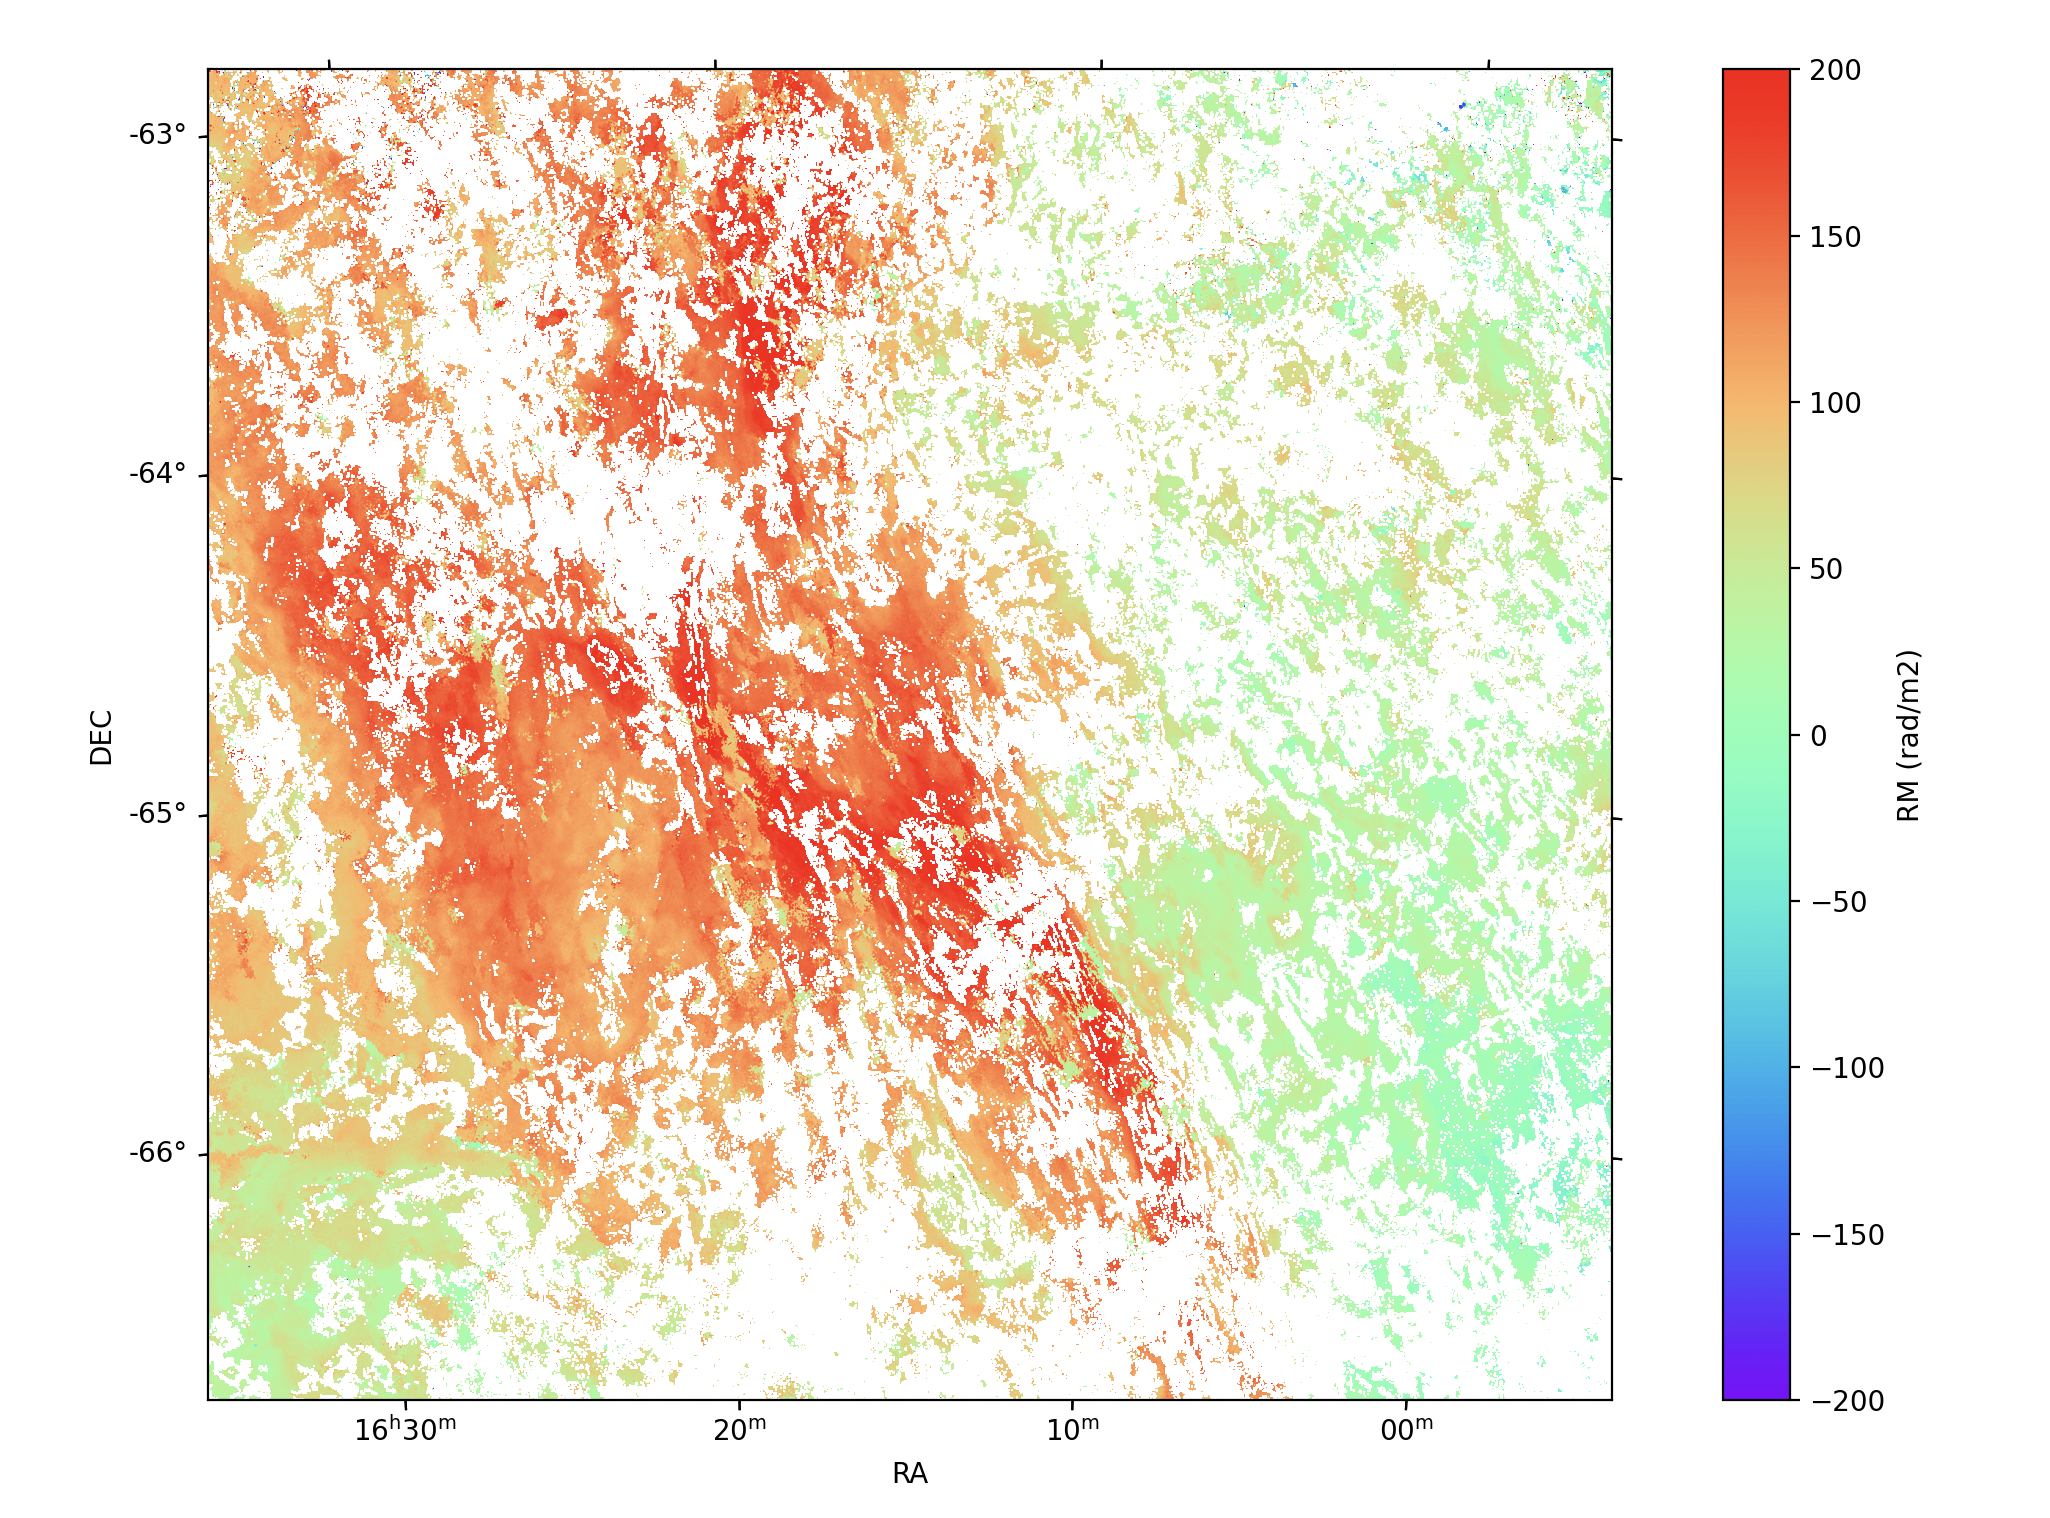
\includegraphics[width=1\linewidth]{Thesis_Template/Figures/1615-64_RM.png}
    \caption{Rotation Measure map of EMU field 1615-64.}
    \label{fig:1615-64 rm}
\end{figure}

\begin{figure}
    \centering
    \includegraphics[width=1\linewidth]{Thesis_Template/Figures/1615-64_PI.png}
    \caption{Polarised Intensity map of EMU field 1615-64.}
    \label{fig:1615-64 pi}
\end{figure}

\begin{figure}
    \centering
    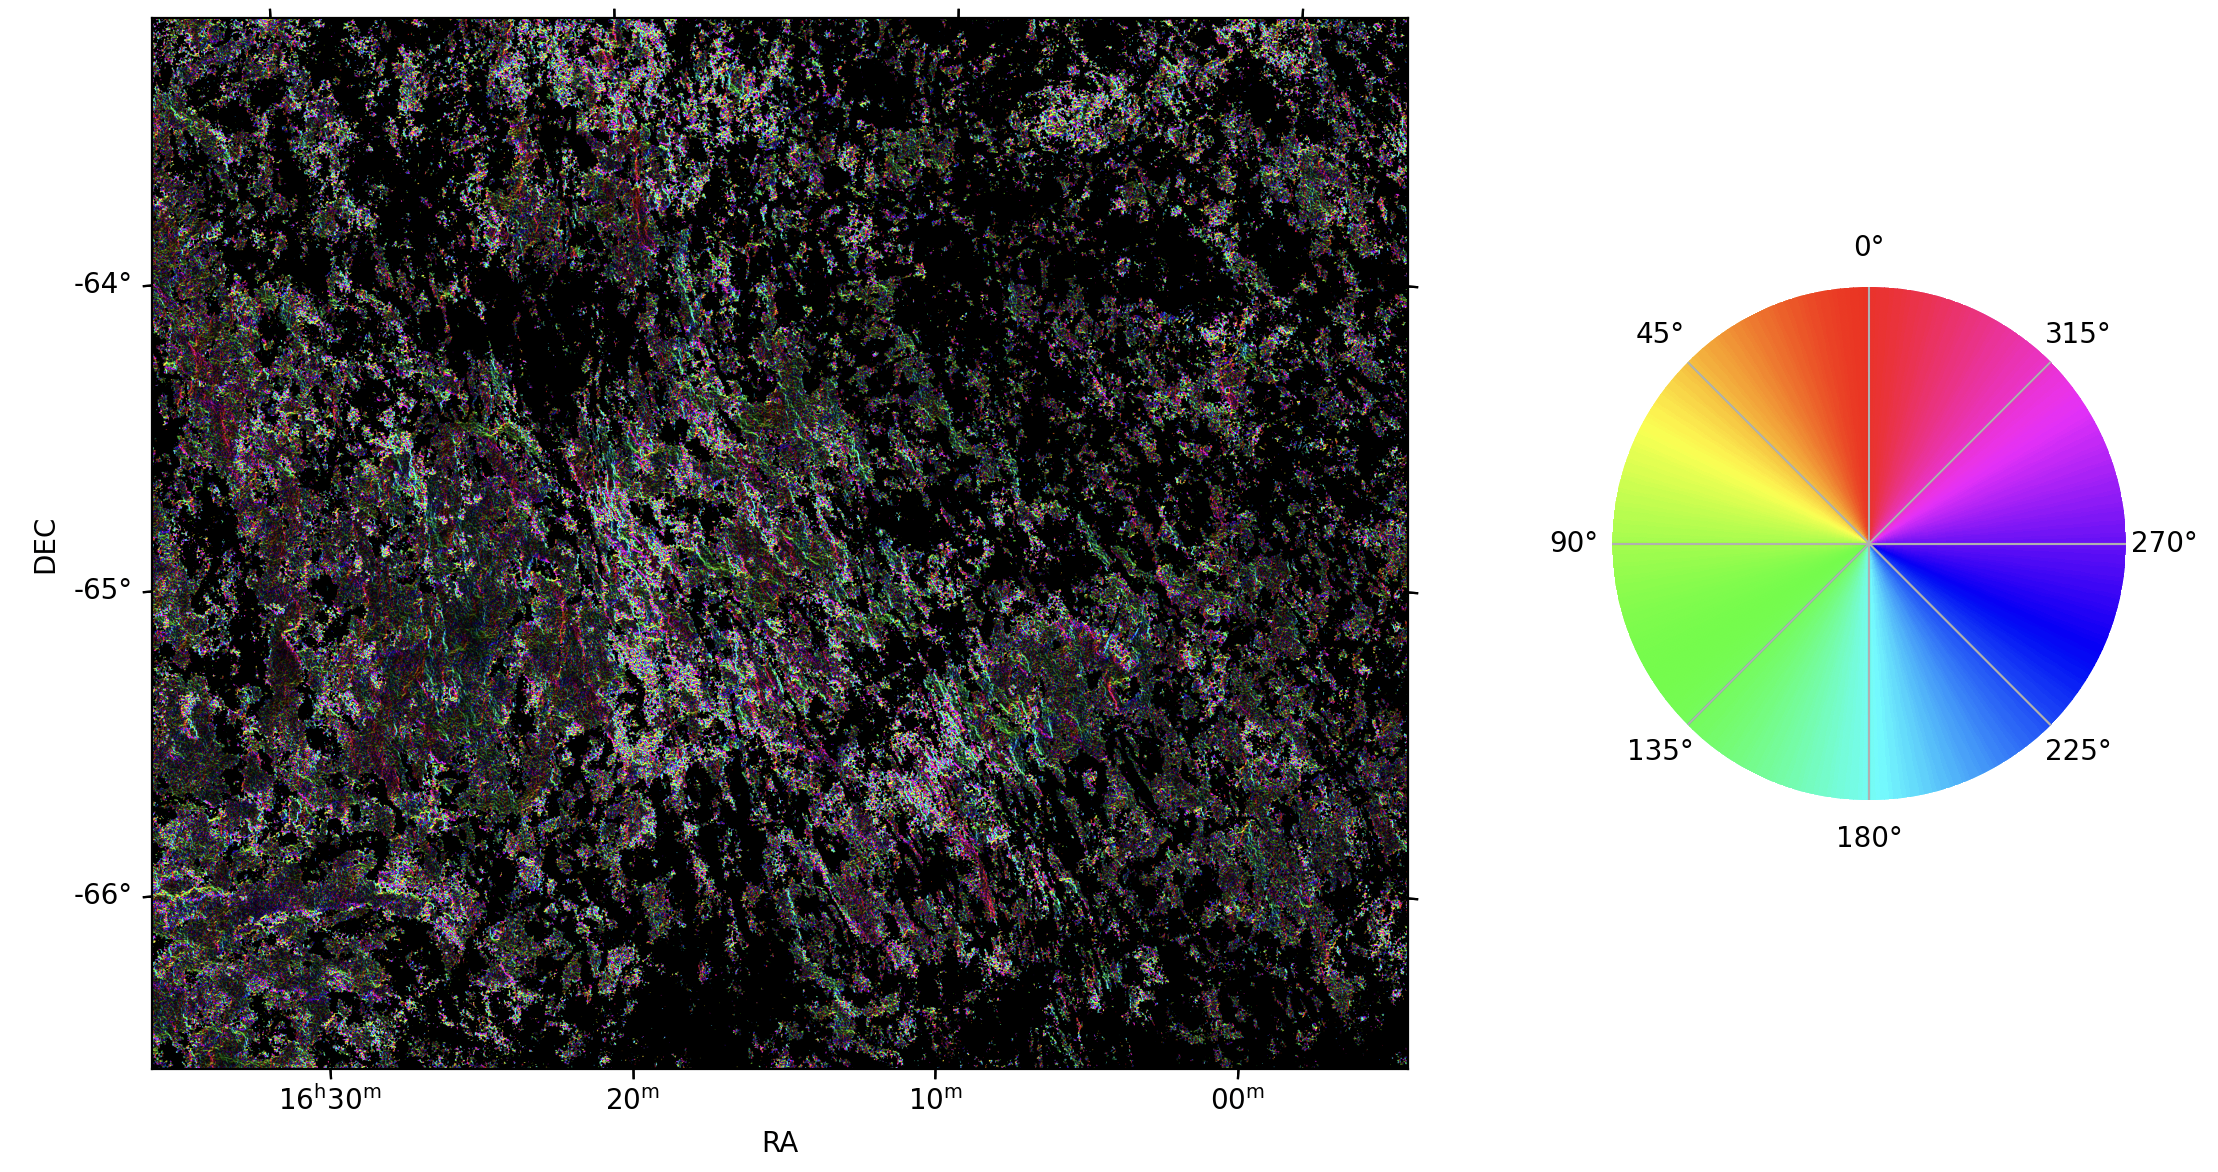
\includegraphics[width=\linewidth]{Thesis_Template/Figures/Hue_3.png}
    \caption{Map of angle and amplitude of the gradient of field EMU1615-64. The colour of the pixel represents the angle of the gradient at that point, and the brightness of the colour represents the amplitude of the gradient at that point, with a higher brightness representing a larger amplitude of gradient. }
    \label{fig:hue}
\end{figure}

\begin{figure}
    \centering
    \begin{subfigure}[b]{0.6\textwidth}
        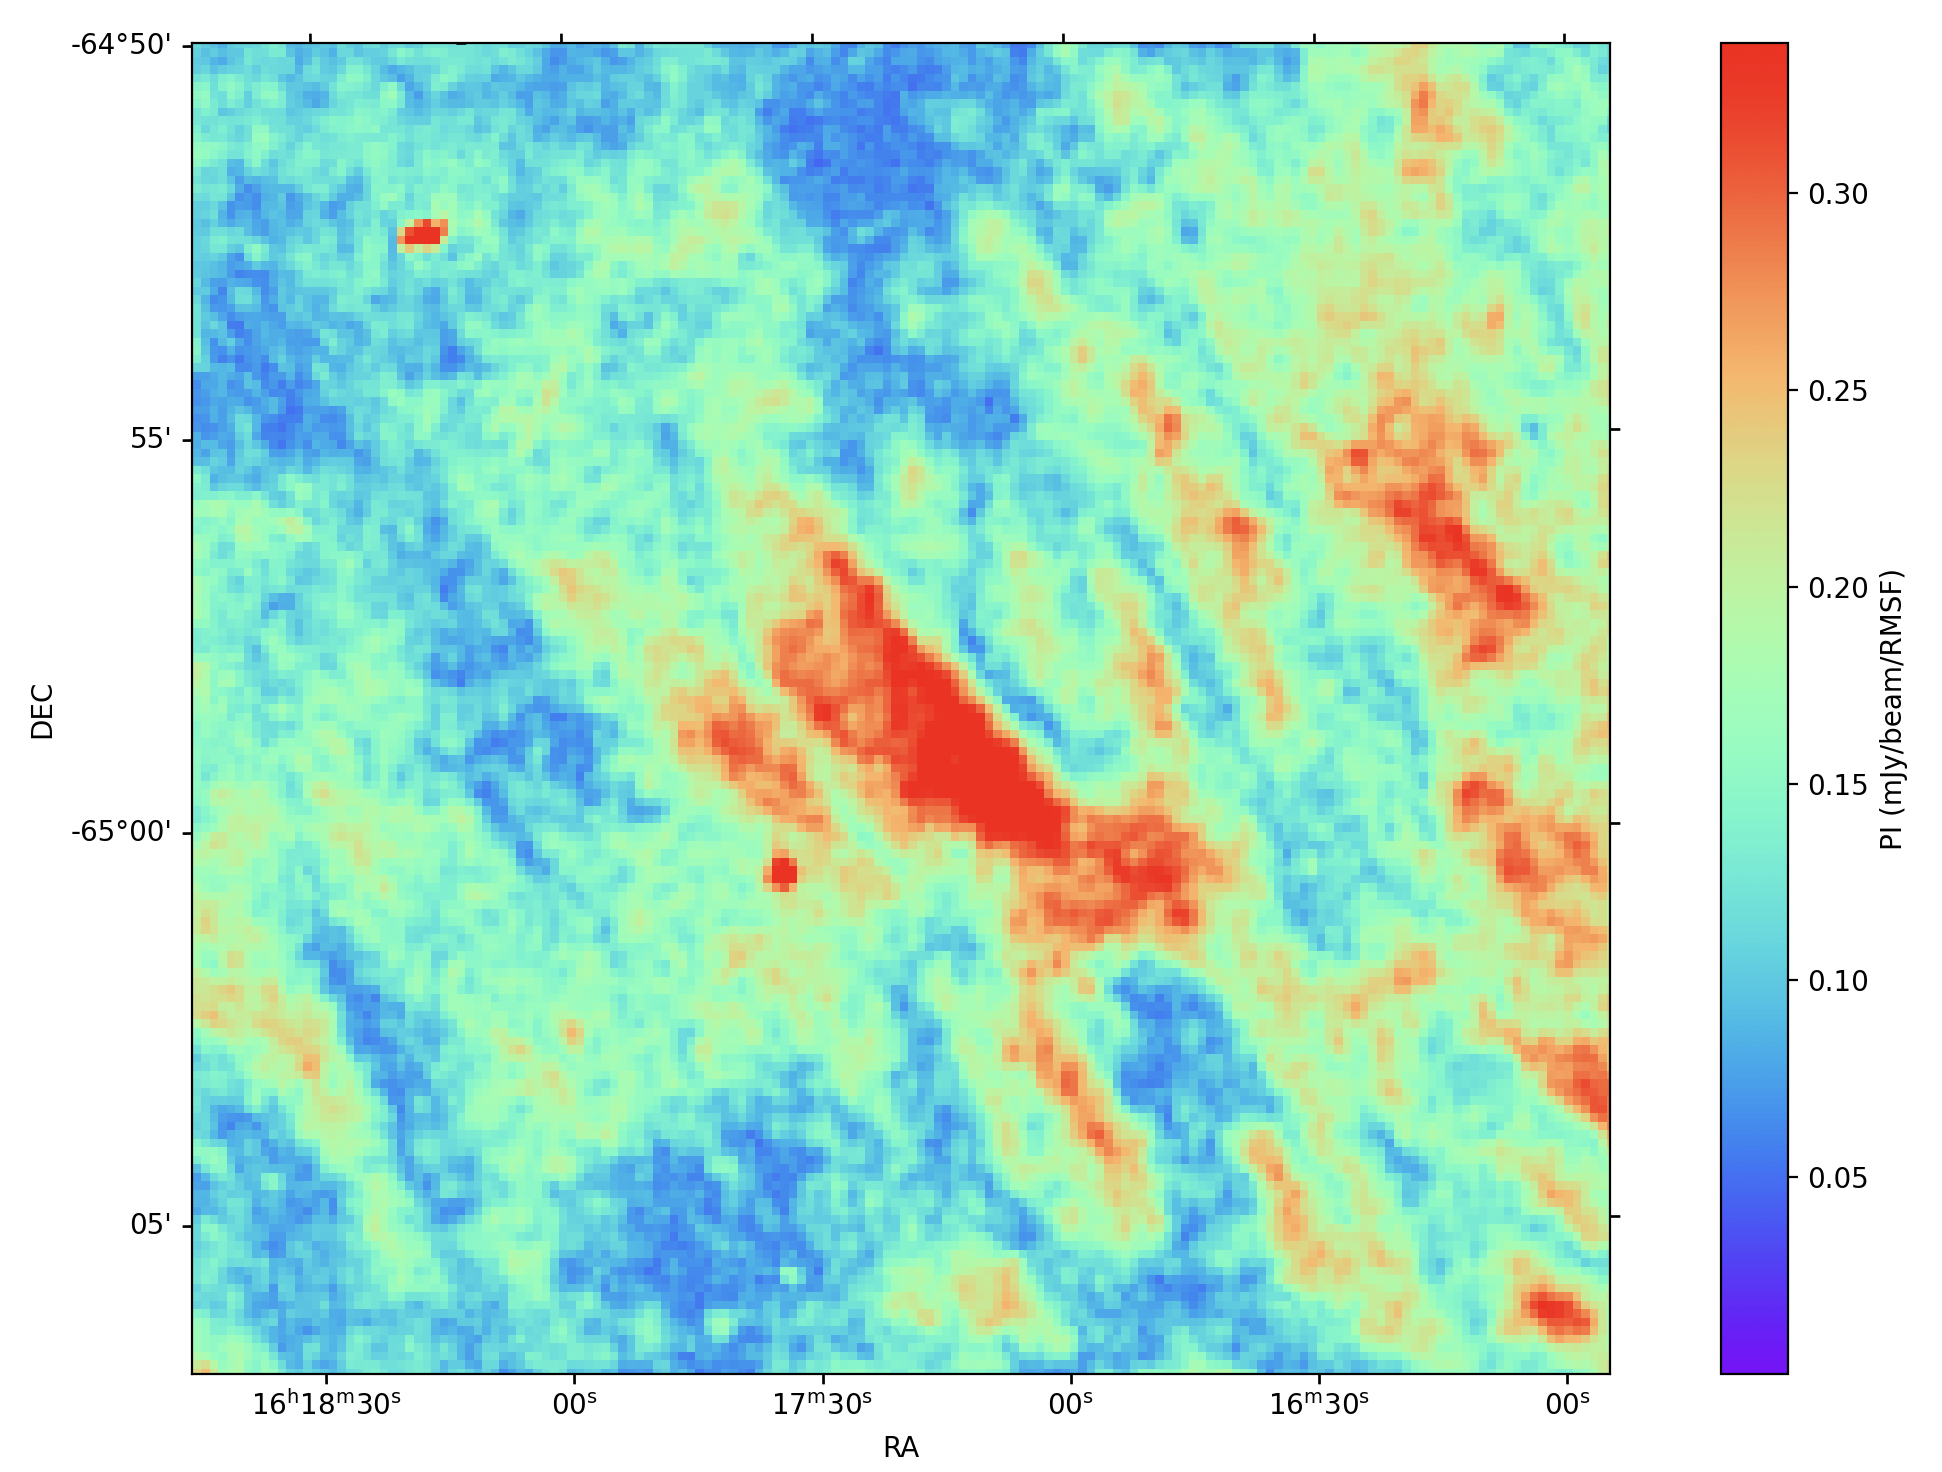
\includegraphics[width=\linewidth]{Thesis_Template/Figures/1615_pi_zoom.png}
        \caption{Zoom in of PI map for field EMU1615-64, with a canal-like feature with a lower PI compared to its surroundings.}
        \label{fig: 1615 pi zoom}
    \end{subfigure}
    \begin{subfigure}[b]{0.6\textwidth}
        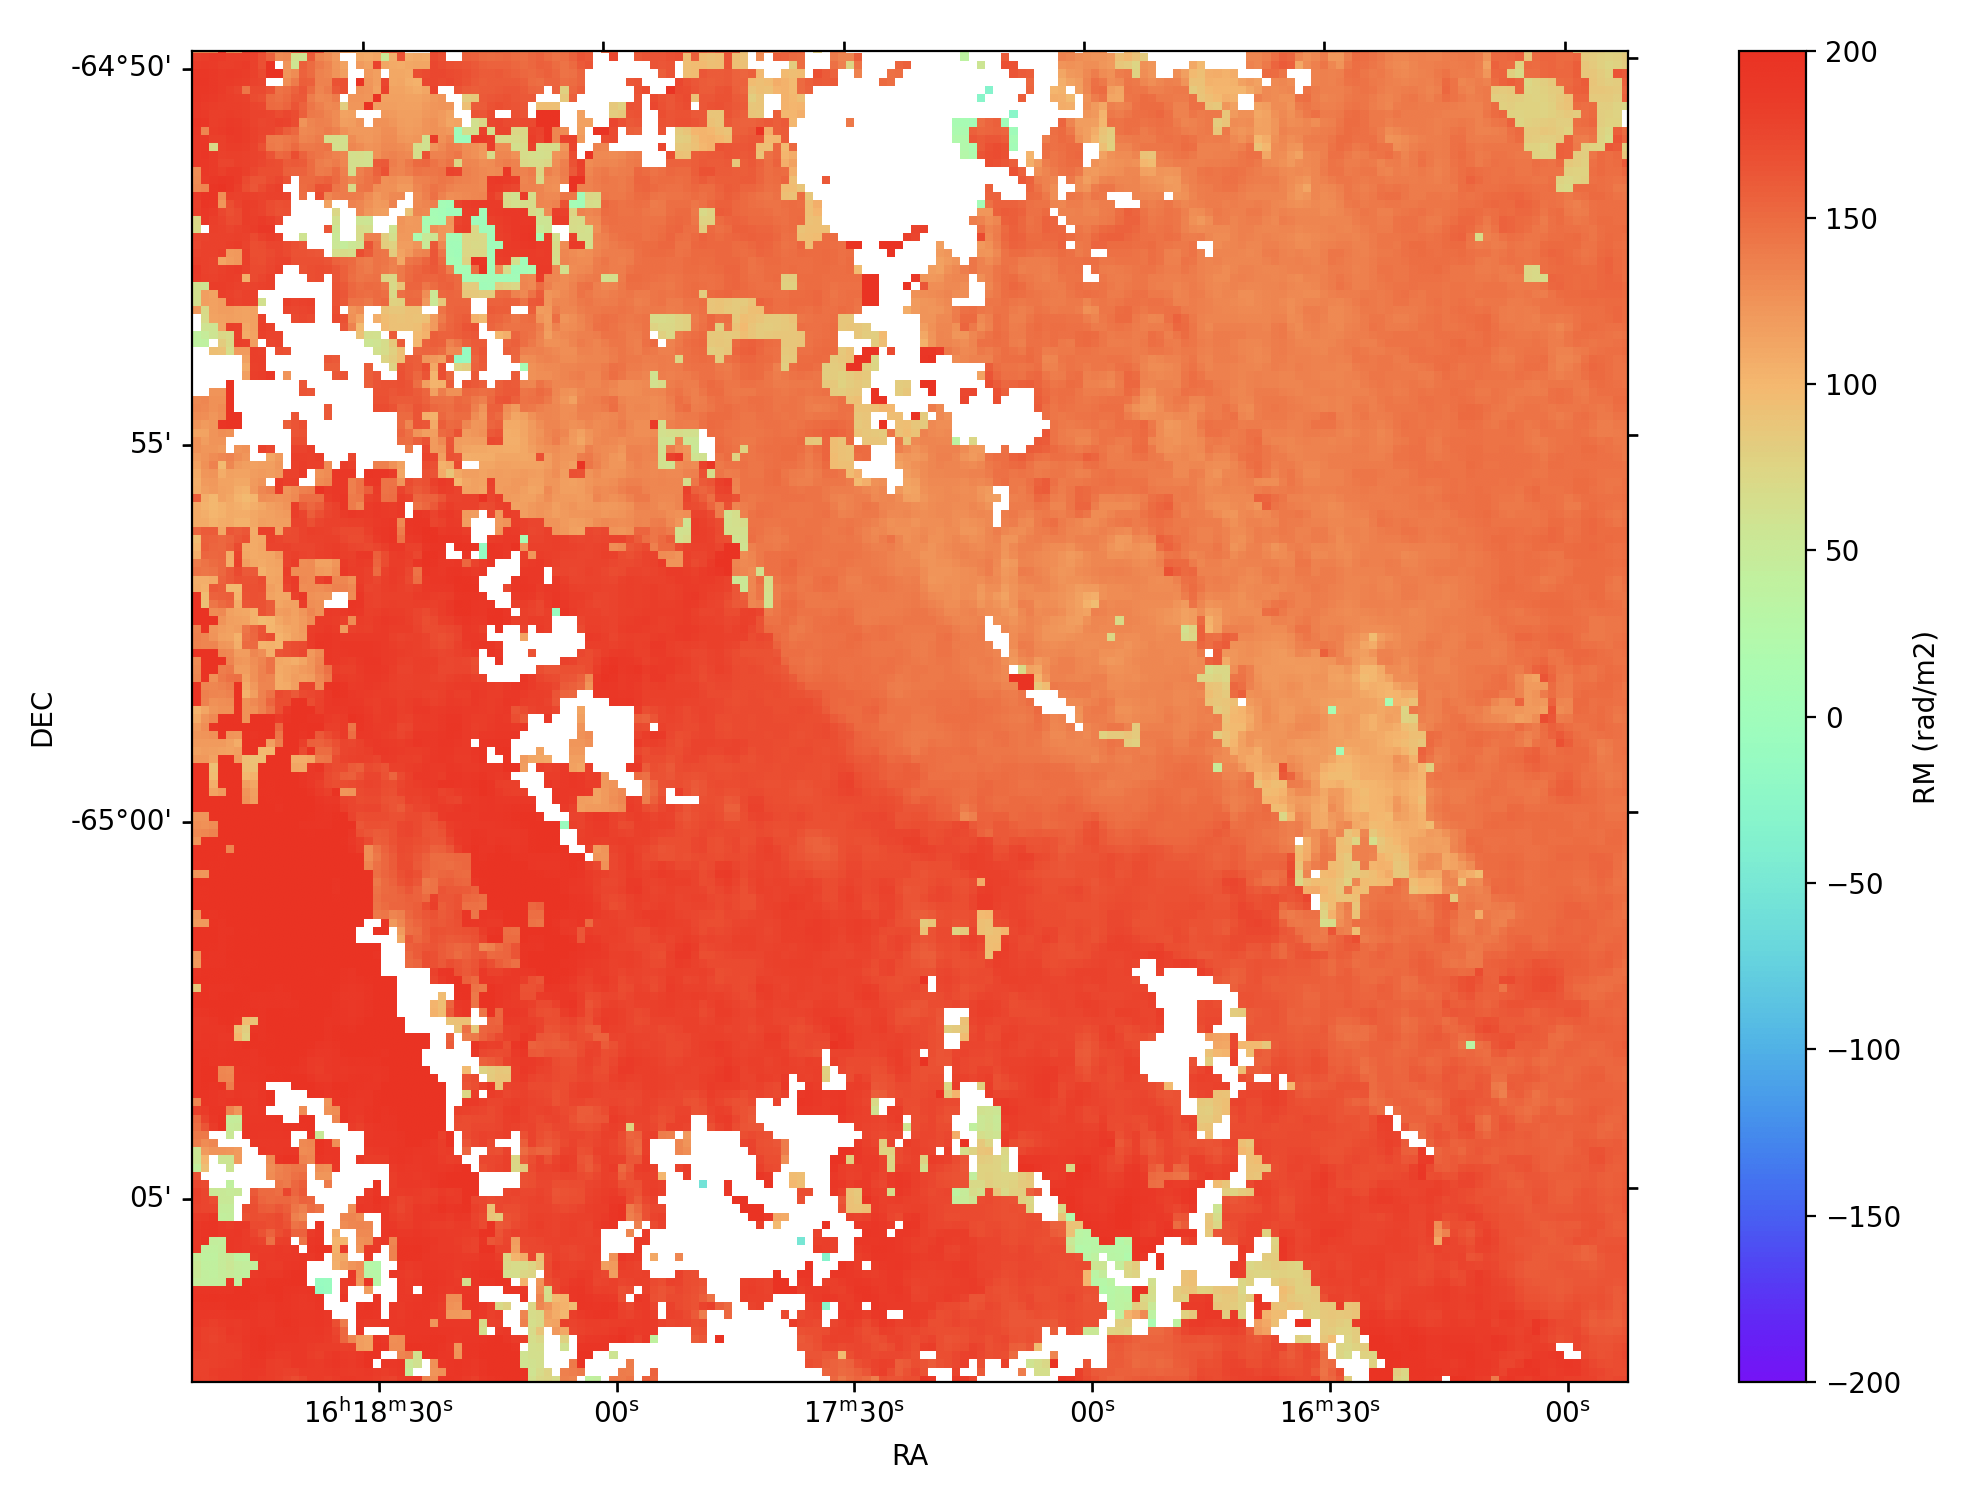
\includegraphics[width=\linewidth]{Thesis_Template/Figures/1615_RM_zoom.png}
        \caption{Zoom in of RM map for field EMU1615-64, showcasing the line of change in RM running across the centre of the image.}
        \label{fig: 1615 rm zoom}
    \end{subfigure}
    \begin{subfigure}[b]{0.7\textwidth}
        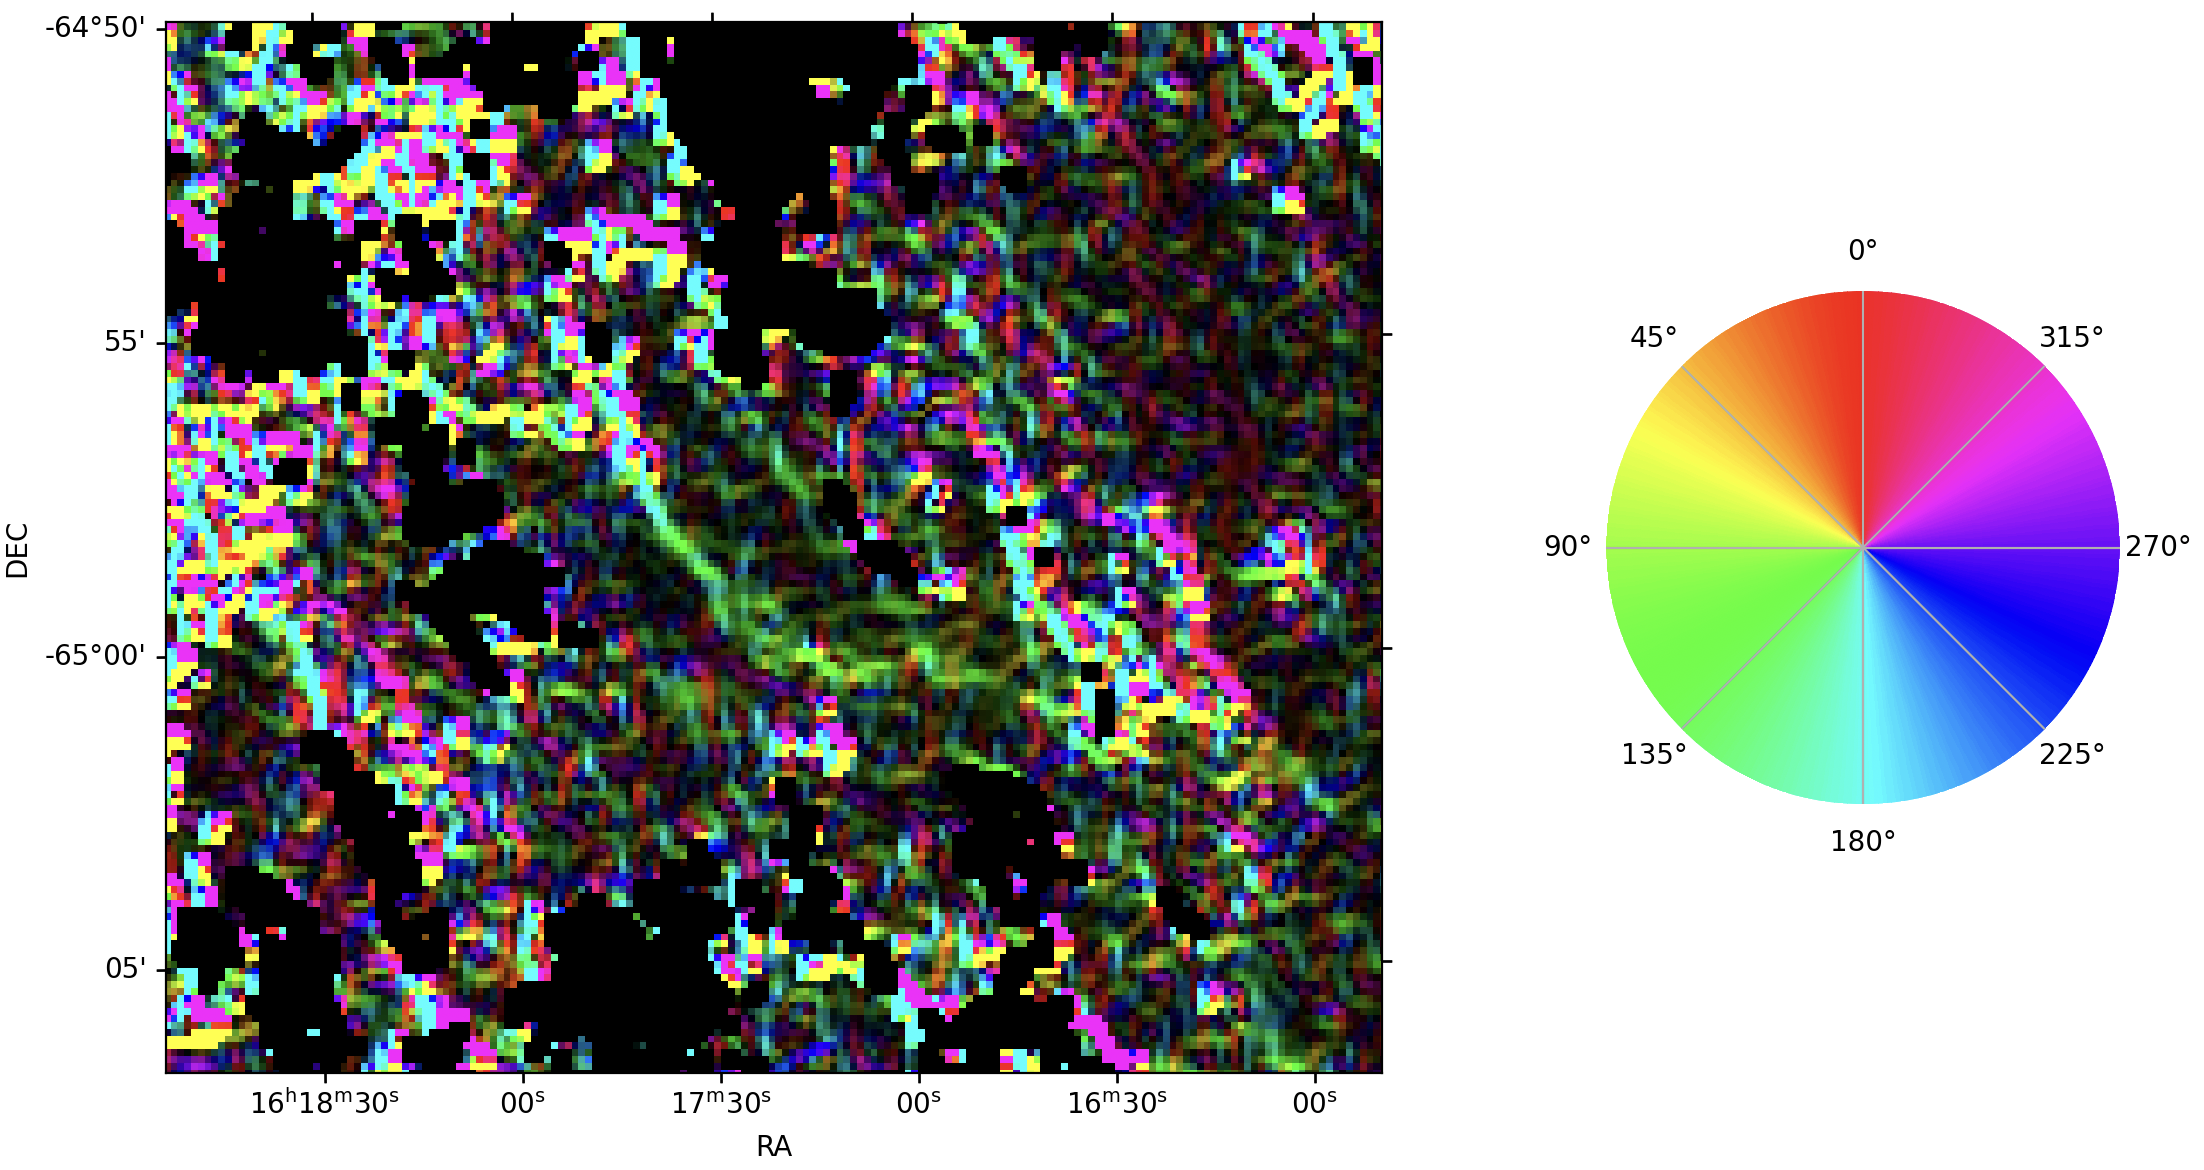
\includegraphics[width=\linewidth]{Thesis_Template/Figures/1615_grad_zoom.png}
        \caption{Zoom in of gradient map for field EMU1615-64, highlighting the central green filament showing a change in gradient of $\sim 135^\circ$.}
        \label{fig: 1615 grad zoom}
    \end{subfigure}
    \caption{Zoom in on feature which can be seen in the centre of all three maps.}
    \label{fig: 1615 zoom}
\end{figure}


Although more work needs to be done to begin to find a conclusive explanation for this phenomena and to be able to create simulations that produce the structure of the diffuse polarisation we are seeing, this work demonstrates the detail in which we are now able to probe with data from POSSUM.


